\documentclass[11pt,a4paper]{article}

\usepackage[a4paper,left=0.62in,right=0.62in,top=0.70in,bottom=0.55in]{geometry}
\usepackage{fontspec}
\setmainfont{NotoSerif}[
  Path=fonts/,
  Extension=.ttf,
  UprightFont=*-Regular,
  BoldFont=*-Bold,
  ItalicFont=*-Italic,
  BoldItalicFont=*-BoldItalic,
  Ligatures=TeX
]
\setsansfont{NotoSerif}[
  Path=fonts/,
  Extension=.ttf,
  UprightFont=*-Regular,
  BoldFont=*-Bold,
  ItalicFont=*-Italic,
  BoldItalicFont=*-BoldItalic,
  Ligatures=TeX
]
\usepackage{amsmath}
\usepackage{graphicx}
\usepackage{xcolor}
\usepackage{array}
\usepackage{caption}
\usepackage{fancyhdr}
\usepackage{hyperref}
\usepackage{enumitem}

\graphicspath{{figures/}}

\definecolor{ink}{HTML}{263342}
\definecolor{coolblue}{HTML}{DCECF6}
\definecolor{coolblue2}{HTML}{C9E5F1}
\definecolor{mint}{HTML}{E4F1EA}
\definecolor{mist}{HTML}{F4FAFC}
\definecolor{lavender}{HTML}{ECEAF7}
\definecolor{softline}{HTML}{B8CAD5}
\definecolor{headergray}{HTML}{A7ADB3}
\definecolor{codebg}{HTML}{F2F7FA}
\definecolor{tablerowgray}{HTML}{F1F3F5}
\definecolor{tablerowwhite}{HTML}{FFFFFF}

\hypersetup{
  colorlinks=true,
  linkcolor=ink,
  urlcolor=ink
}

\pagestyle{fancy}
\fancyhf{}
\lhead{\footnotesize\itshape\textcolor{headergray}{AI-Based CPB Pump Control}}
\rhead{\footnotesize\itshape\textcolor{headergray}{Sawab Hussein}}
\cfoot{\thepage}
\renewcommand{\headrulewidth}{0.35pt}
\makeatletter
\renewcommand{\headrule}{%
  {\color{softline}\hrule\@height\headrulewidth\@width\headwidth}%
  \vskip-\headrulewidth
}
\makeatother

\setlength{\parindent}{0pt}
\setlength{\parskip}{2pt}
\setlength{\headheight}{15pt}
\setlength{\headsep}{14pt}
\setlist[itemize]{leftmargin=1.3em, itemsep=0.5pt, topsep=1pt}
\renewcommand{\arraystretch}{1.16}
\captionsetup{font=small, labelfont=bf, skip=2pt}
\AtBeginDocument{%
  \setlength{\abovedisplayskip}{4pt}%
  \setlength{\belowdisplayskip}{4pt}%
  \setlength{\abovedisplayshortskip}{3pt}%
  \setlength{\belowdisplayshortskip}{3pt}%
}
\makeatletter
\renewcommand*\l@section{\@dottedtocline{1}{0em}{1.8em}}
\renewcommand*\l@subsection{\@dottedtocline{2}{1.8em}{2.8em}}
\makeatother

\newcommand{\term}[1]{\textit{#1}}
\newcommand{\rowbox}[2]{%
  \noindent\colorbox{#1}{%
    \parbox{\dimexpr\linewidth-2\fboxsep\relax}{#2}%
  }\par\vspace{1pt}%
}
\newcommand{\fourcolrow}[5]{%
  \rowbox{#1}{%
    \setlength{\tabcolsep}{2pt}%
    \begin{tabular}{@{}p{0.22\linewidth}p{0.24\linewidth}p{0.24\linewidth}p{0.24\linewidth}@{}}
      #2 & #3 & #4 & #5
    \end{tabular}%
  }%
}
\newcommand{\rulecolrow}[5]{%
  \rowbox{#1}{%
    \setlength{\tabcolsep}{2pt}%
    \begin{tabular}{@{}p{0.22\linewidth}p{0.18\linewidth}p{0.22\linewidth}p{0.18\linewidth}@{}}
      #2 & #3 & #4 & #5
    \end{tabular}%
  }%
}
\newcommand{\threecolrow}[4]{%
  \rowbox{#1}{%
    \setlength{\tabcolsep}{2pt}%
    \begin{tabular}{@{}p{0.16\linewidth}p{0.58\linewidth}p{0.18\linewidth}@{}}
      #2 & #3 & #4
    \end{tabular}%
  }%
}
\newcommand{\rulecodeblock}{%
  \noindent\colorbox{codebg}{%
    \parbox{\dimexpr\linewidth-2\fboxsep\relax}{%
      \small
      1. \textbf{IF} \(\Delta P\) is low AND \(Q\) is low \textbf{THEN} Speed = fast\par
      2. \textbf{IF} \(\Delta P\) is low AND \(Q\) is medium \textbf{THEN} Speed = medium\par
      3. \textbf{IF} \(\Delta P\) is low AND \(Q\) is high \textbf{THEN} Speed = slow\par
      4. \textbf{IF} \(\Delta P\) is medium AND \(Q\) is low \textbf{THEN} Speed = medium\par
      5. \textbf{IF} \(\Delta P\) is medium AND \(Q\) is medium \textbf{THEN} Speed = medium\par
      6. \textbf{IF} \(\Delta P\) is medium AND \(Q\) is high \textbf{THEN} Speed = slow\par
      7. \textbf{IF} \(\Delta P\) is high AND \(Q\) is low \textbf{THEN} Speed = medium\par
      8. \textbf{IF} \(\Delta P\) is high AND \(Q\) is medium \textbf{THEN} Speed = medium\par
      9. \textbf{IF} \(\Delta P\) is high AND \(Q\) is high \textbf{THEN} Speed = slow%
    }%
  }%
}

\begin{document}
\thispagestyle{empty}

\begin{center}
  
\includegraphics[width=0.405\linewidth]{AUK-logo.png}\\[16pt]
  \parbox{0.9\linewidth}{\centering
    {\LARGE\bfseries\textcolor{ink}{AI-Based Smart Cardiopulmonary Blood Flow Control System}}\\[3pt]
    {\large\textcolor{ink}{Fuzzy Logic Controller Report}}%
  }\\[6pt]
  \begin{tabular}{>{\bfseries}r l}
    Student Name: & Sawab Hussein\\
    Instructor: & Dr. Omar Abdulghafoor\\
    Course: & Artificial Intelligence, Spring 2026\\
  \end{tabular}
\end{center}

\vspace{2pt}
\tableofcontents
\clearpage

\section{Problem Statement}

A cardiopulmonary bypass rotary pump must maintain safe blood flow by adjusting the pump speed \(N\). The required operating point is
\[
  \Delta P = 84\ \text{mmHg}, \qquad Q = 6\ \text{L/min}.
\]
The work completed for this project was to convert the assignment rule table into a complete fuzzy controller, evaluate the controller at the required operating point, draw the intermediate and final fuzzy sets, and compute the crisp rotary-pump speed. The implementation in \path{fuzzy_cpb_controller.py} defines the membership functions, stores the nine IF--THEN rules, performs Mamdani inference, and applies centroid defuzzification by numerical integration.

The controller uses the standard Mamdani sequence: fuzzify the two inputs, compute each rule firing strength with the logical AND operator as a minimum, clip each output membership function by its rule strength, combine all output clips with a maximum operator, and finally defuzzify the aggregated output set.

\section{Membership Functions and Rules}

The triangular membership functions were read from the assignment figures. The universes are \(Q\in[0,10]\) L/min, \(\Delta P\in[50,150]\) mmHg, and \(N\in[2800,3200]\) rpm; the vertices used in the implementation are summarized below.

\begin{table}[h]
\centering
\caption{Triangular membership vertices used by the controller.}
\fourcolrow{coolblue2}{\textbf{Variable}}{\textbf{Low / Slow}}{\textbf{Medium}}{\textbf{High / Fast}}
\fourcolrow{tablerowgray}{\textbf{Blood flow \(Q\) (L/min)}}{\((0,\ 3.5,\ 6)\)}{\((3.5,\ 6,\ 8.5)\)}{\((6,\ 8.5,\ 10)\)}
\fourcolrow{tablerowwhite}{\textbf{Delta pressure \(\Delta P\) (mmHg)}}{\((50,\ 72,\ 100)\)}{\((72,\ 100,\ 120)\)}{\((100,\ 120,\ 142)\)}
\fourcolrow{tablerowgray}{\textbf{Pump speed \(N\) (rpm)}}{\((2800,\ 2900,\ 3000)\)}{\((2900,\ 3000,\ 3100)\)}{\((3000,\ 3100,\ 3200)\)}
\end{table}

\begin{center}
  \centering
  \begin{minipage}{0.47\linewidth}
    \centering
    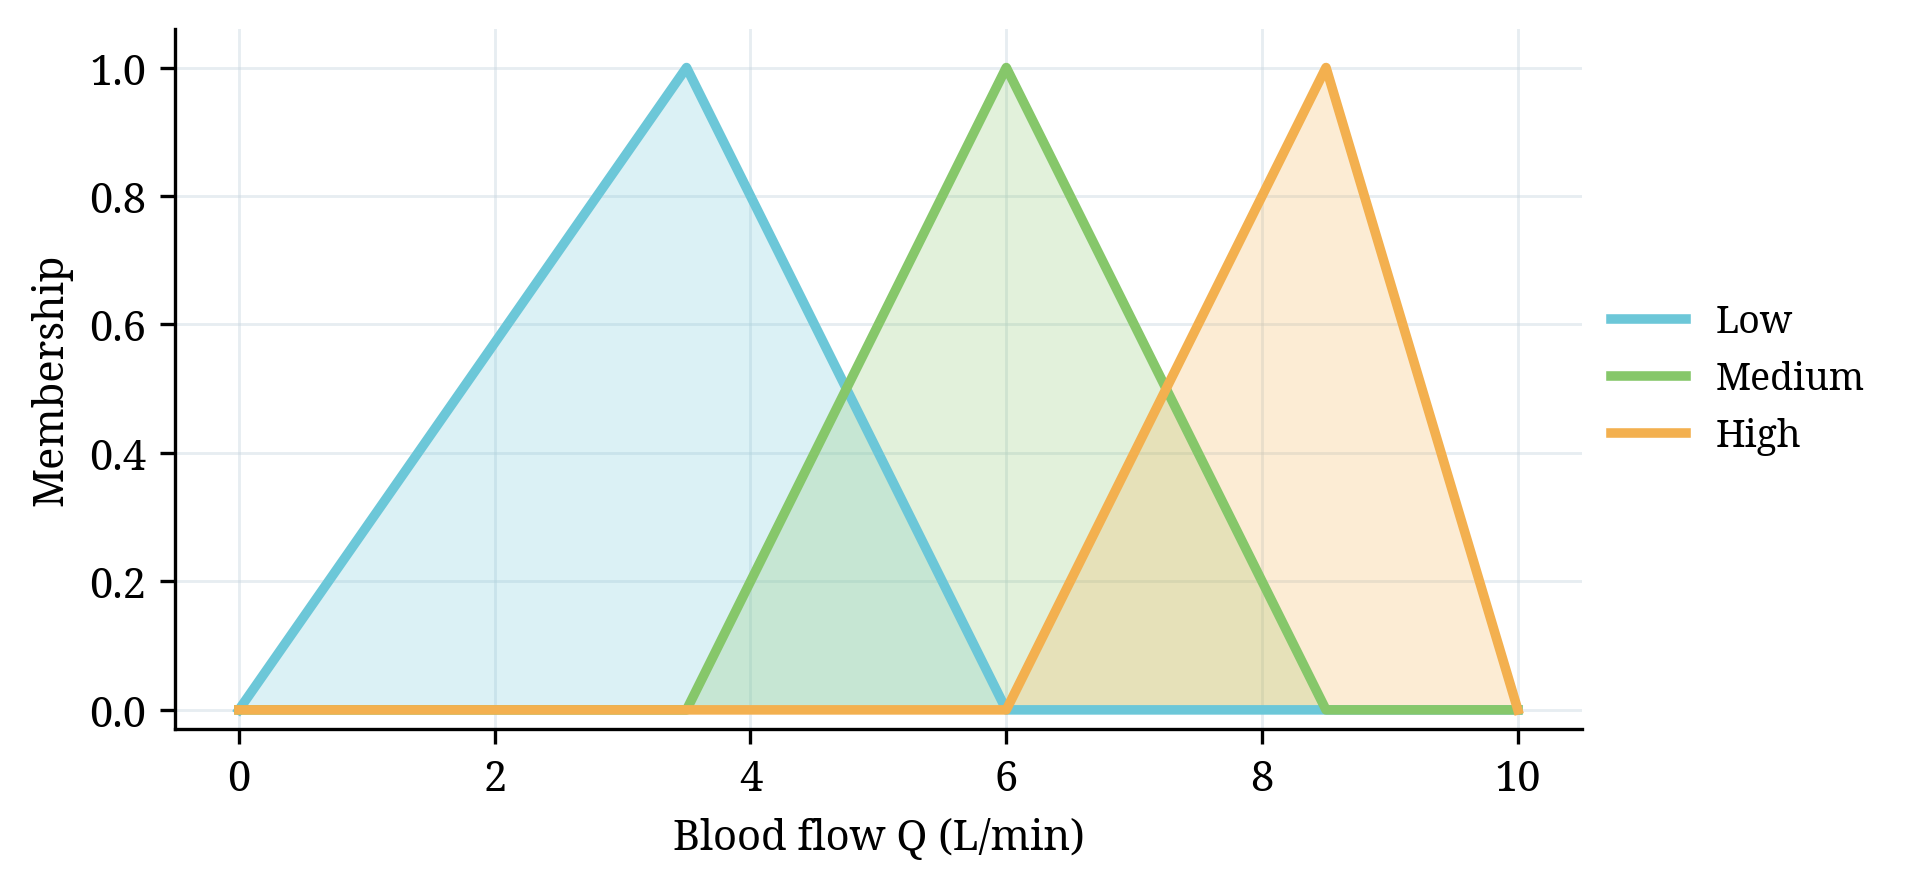
\includegraphics[width=\linewidth]{membership_flow.png}
  \end{minipage}\hspace{0.025\linewidth}
  \begin{minipage}{0.47\linewidth}
    \centering
    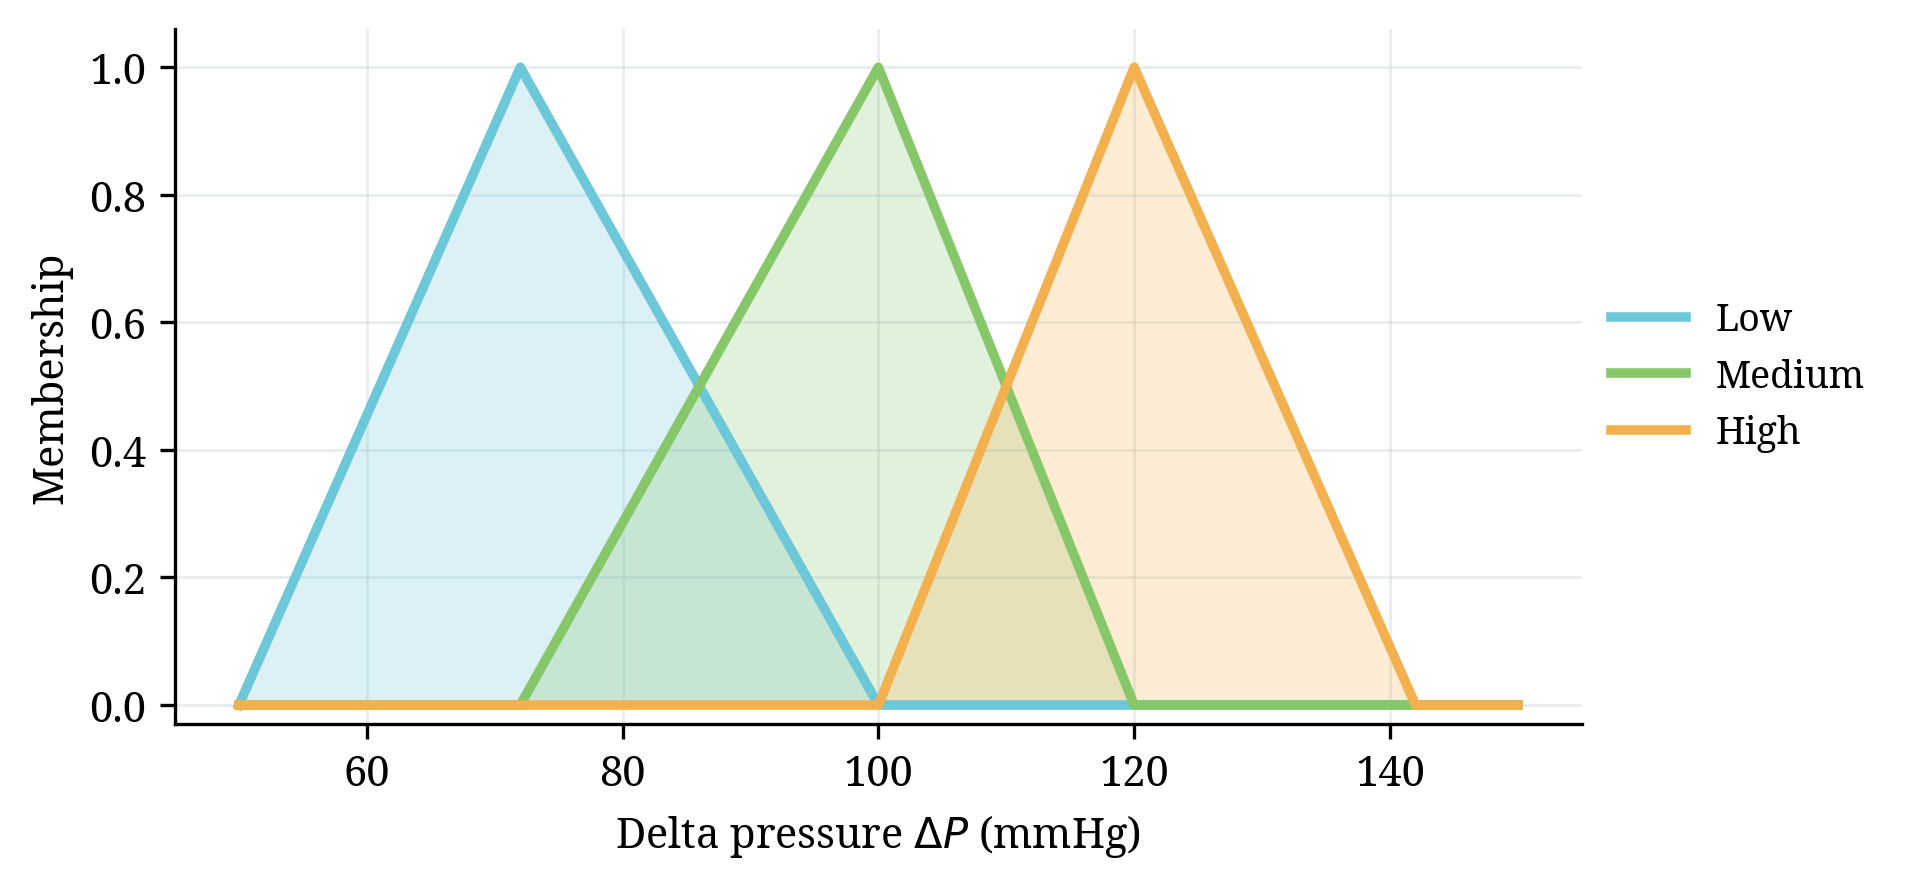
\includegraphics[width=\linewidth]{membership_pressure.png}
  \end{minipage}\\[4pt]
  \begin{minipage}{0.47\linewidth}
    \centering
    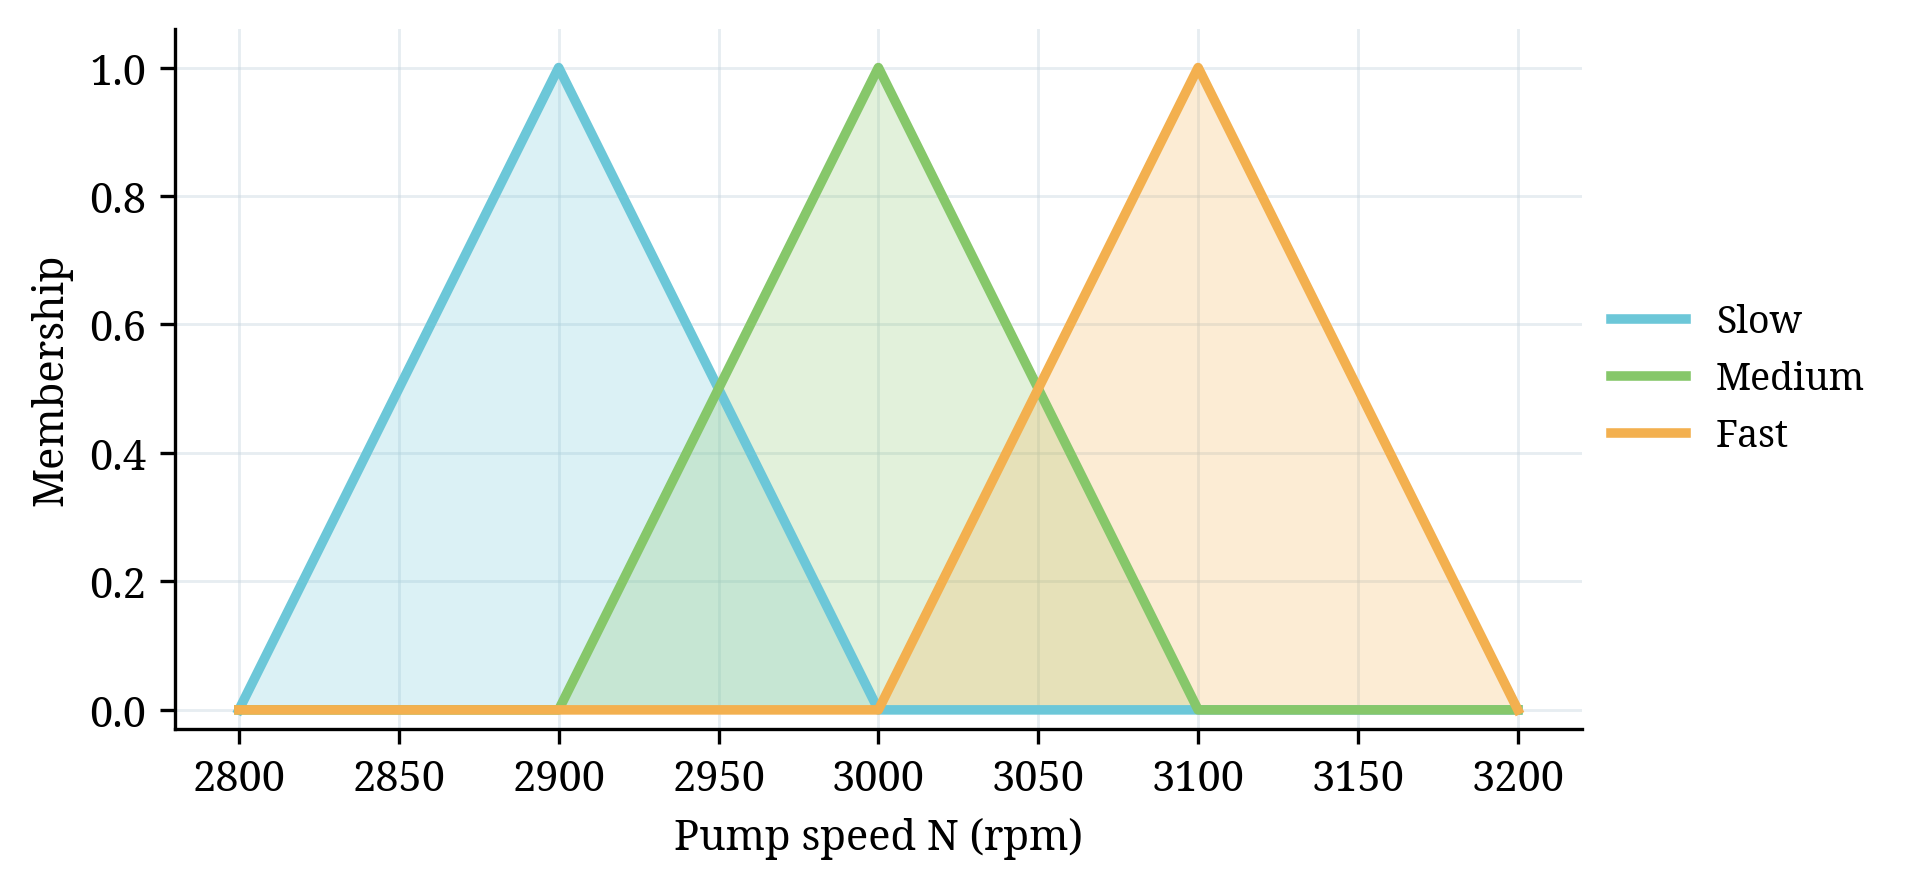
\includegraphics[width=\linewidth]{membership_speed.png}
  \end{minipage}
  \captionof{figure}{Membership functions for flow, pressure difference, and pump speed.}
\end{center}

Figure 1 is the controller definition in graphical form. The first two panels show how measured flow and pressure are translated into linguistic values, while the third panel shows the possible linguistic pump-speed outputs. These curves are the numerical basis used by the Python file when it calculates memberships for \(Q=6\) and \(\Delta P=84\).

\begin{table}[h]
\centering
\caption{Fuzzy rule base used for the rotary pump controller.}
\rulecolrow{coolblue2}{\textbf{\(\Delta P \backslash Q\)}}{\textbf{Low Flow}}{\textbf{Medium Flow}}{\textbf{High Flow}}
\rulecolrow{tablerowgray}{\textbf{Low \(\Delta P\)}}{Fast}{Medium}{Slow}
\rulecolrow{tablerowwhite}{\textbf{Medium \(\Delta P\)}}{Medium}{Medium}{Slow}
\rulecolrow{tablerowgray}{\textbf{High \(\Delta P\)}}{Medium}{Medium}{Slow}
\end{table}

\subsection*{Explicit IF--THEN Rules}
\addcontentsline{toc}{subsection}{Explicit IF--THEN Rules}

\rulecodeblock

\section{Inference at the Required Operating Point}

The input \(Q=6\) lies exactly at the peak of the medium-flow triangle. Therefore, the flow input belongs completely to the medium set and has zero membership in the low and high sets. The pressure value \(\Delta P=84\) lies in the overlap between low and medium pressure, so both pressure labels are partially active.

For \(Q=6\), the medium-flow set is fully active:
\[
  \mu_{Q,\text{low}}(6)=0,\qquad
  \mu_{Q,\text{medium}}(6)=1,\qquad
  \mu_{Q,\text{high}}(6)=0.
\]
For \(\Delta P=84\), the two active pressure memberships are
\[
  \mu_{\Delta P,\text{low}}(84)=\frac{100-84}{100-72}=0.571,
  \qquad
  \mu_{\Delta P,\text{medium}}(84)=\frac{84-72}{100-72}=0.429.
\]

Only two rules fire with nonzero strength:

\begin{table}[h]
\centering
\caption{Nonzero rule activations.}
\threecolrow{coolblue2}{\textbf{Rule}}{\textbf{Consequent}}{\textbf{Firing strength}}
\threecolrow{tablerowgray}{\textbf{R2}}{Low \(\Delta P\), Medium \(Q\): Speed is Medium}{\(0.571\)}
\threecolrow{tablerowwhite}{\textbf{R5}}{Medium \(\Delta P\), Medium \(Q\): Speed is Medium}{\(0.429\)}
\end{table}

Both active rules point to the same consequent, so the aggregated output is simply the medium-speed membership function clipped at
\[
  \alpha_{\text{medium}}=\max(0.571,\ 0.429)=0.571.
\]
The remaining rules have zero firing strength because one of their required input labels has zero membership at this operating point.

Figure 2 visualizes the full rule matrix and confirms that only two cells are active: low pressure with medium flow, and medium pressure with medium flow. Figure 3 then shows the consequence of these active rules: the medium-speed output set is clipped at \(0.571\), while the slow and fast output sets do not contribute to the aggregate. The vertical dashed line marks the centroid of the aggregated output.

\begin{center}
  \centering
  \begin{minipage}{0.40\linewidth}
    \centering
    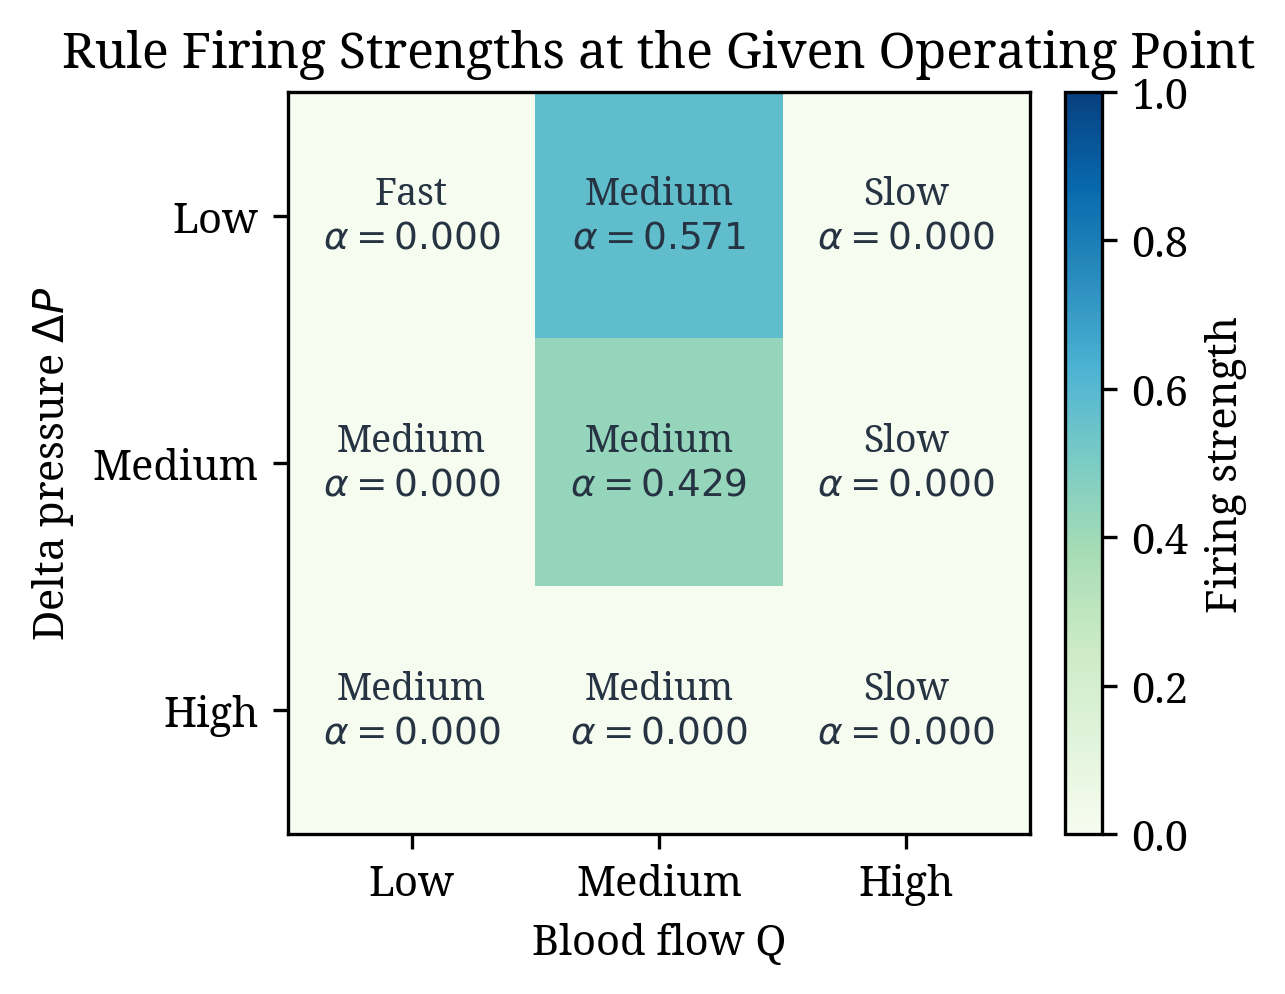
\includegraphics[width=\linewidth]{rule_activation.png}
    \captionof{figure}{Rule firing strengths.}
  \end{minipage}\hfill
  \begin{minipage}{0.42\linewidth}
    \centering
    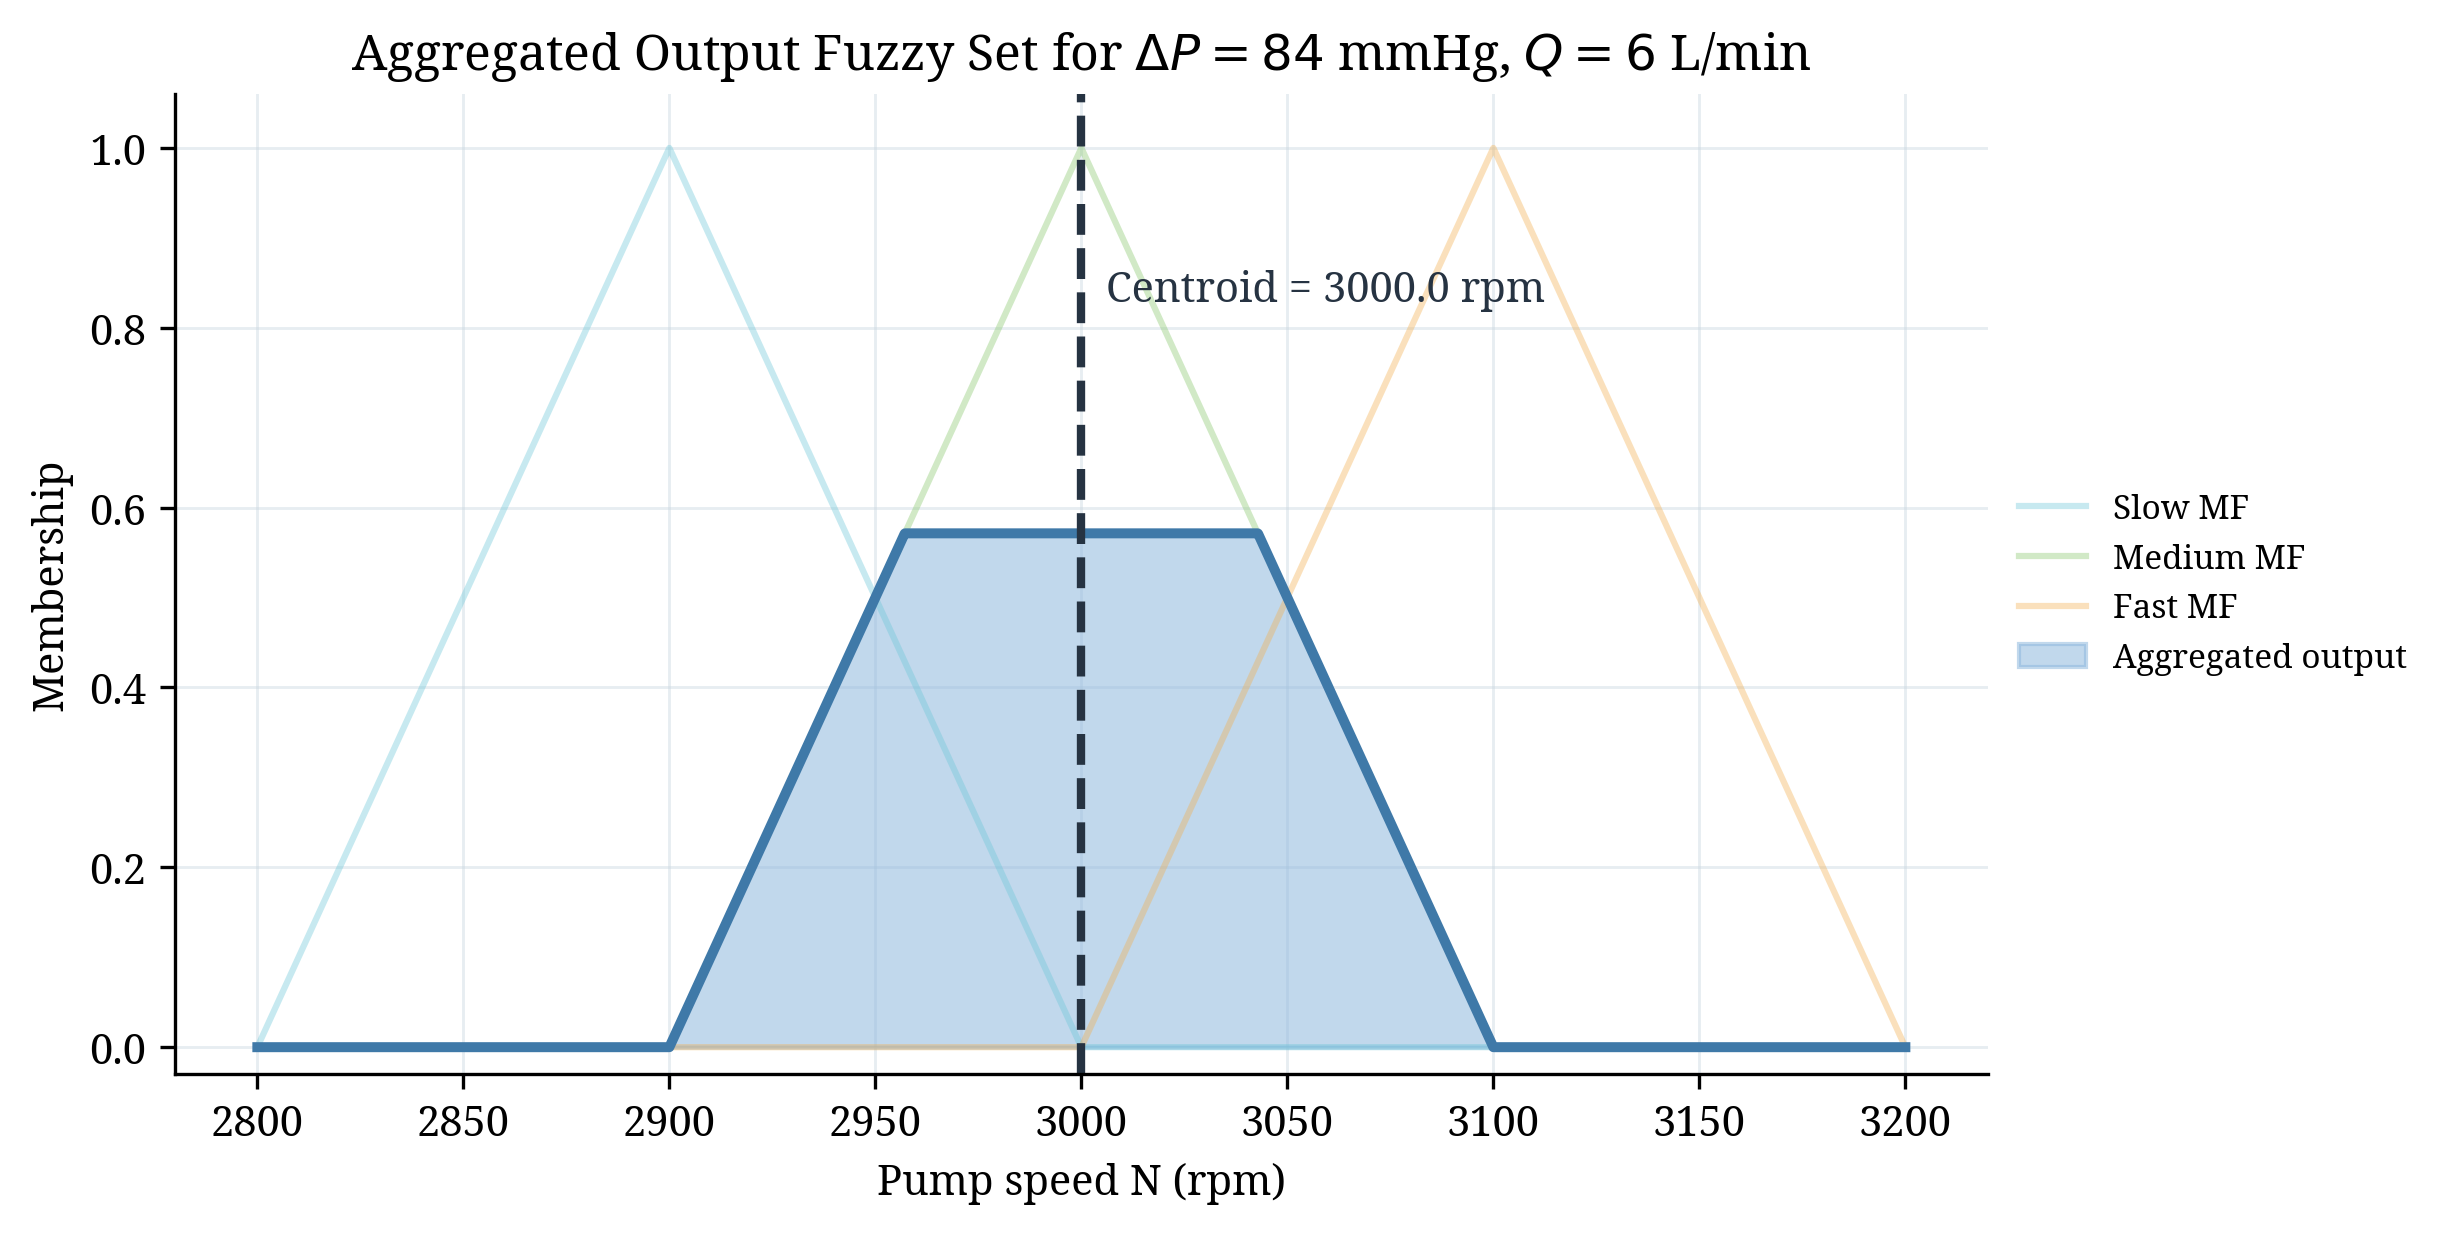
\includegraphics[width=\linewidth]{aggregated_output.png}
    \captionof{figure}{Aggregated output fuzzy set.}
  \end{minipage}
\end{center}

\section{Centroid Defuzzification}

The centroid method computes
\[
  N^\ast =
  \frac{\int_{2800}^{3200} n\,\mu_{\text{agg}}(n)\,dn}
       {\int_{2800}^{3200} \mu_{\text{agg}}(n)\,dn}.
\]
For this operating point, the active output is the medium-speed triangle clipped at
\(\alpha=0.571=4/7\). The unclipped medium-speed set is centered at \(3000\) rpm and
has the vertices \((2900,0)\), \((3000,1)\), and \((3100,0)\). The clipping level
intersects the triangle at
\[
  n_L = 2900 + 100\left(\frac{4}{7}\right)=2957.143,
  \qquad
  n_R = 3100 - 100\left(\frac{4}{7}\right)=3042.857.
\]
Therefore, the aggregated membership function is
\[
\mu_{\text{agg}}(n)=
\begin{cases}
  \dfrac{n-2900}{100}, & 2900\le n\le 2957.143,\\[4pt]
  \dfrac{4}{7}, & 2957.143\le n\le 3042.857,\\[4pt]
  \dfrac{3100-n}{100}, & 3042.857\le n\le 3100,\\[4pt]
  0, & \text{otherwise}.
\end{cases}
\]

First, evaluate the denominator, which is the area under the clipped output set:
\[
\begin{aligned}
  A
  &= \int_{2900}^{2957.143}\frac{n-2900}{100}\,dn
   + \int_{2957.143}^{3042.857}\frac{4}{7}\,dn
   + \int_{3042.857}^{3100}\frac{3100-n}{100}\,dn \\[2pt]
  &= 16.327 + 48.980 + 16.327 \\
  &= 81.633.
\end{aligned}
\]
Next, evaluate the numerator, which is the first moment of the clipped output set:
\[
\begin{aligned}
  M
  &= \int_{2900}^{2957.143}n\left(\frac{n-2900}{100}\right)\,dn
   + \int_{2957.143}^{3042.857}n\left(\frac{4}{7}\right)\,dn
   + \int_{3042.857}^{3100}n\left(\frac{3100-n}{100}\right)\,dn \\[2pt]
  &= \left[\frac{n^3}{300}-\frac{29n^2}{2}\right]_{2900}^{2957.143}
   + \left[\frac{2n^2}{7}\right]_{2957.143}^{3042.857}
   + \left[\frac{31n^2}{2}-\frac{n^3}{300}\right]_{3042.857}^{3100} \\[2pt]
  &= 47{,}968.902 + 146{,}938.776 + 49{,}990.282 \\
  &= 244{,}897.959.
\end{aligned}
\]

\newpage

Finally, divide the first moment by the area:
\[
  N^\ast=\frac{M}{A}
  =\frac{244{,}897.959}{81.633}
  =\boxed{3000.0\ \text{rpm}}.
\]
The exact arithmetic gives the same value because
\(M=12{,}000{,}000/49\) and \(A=4000/49\), so the ratio is exactly \(3000\).

\begin{center}
  \centering
  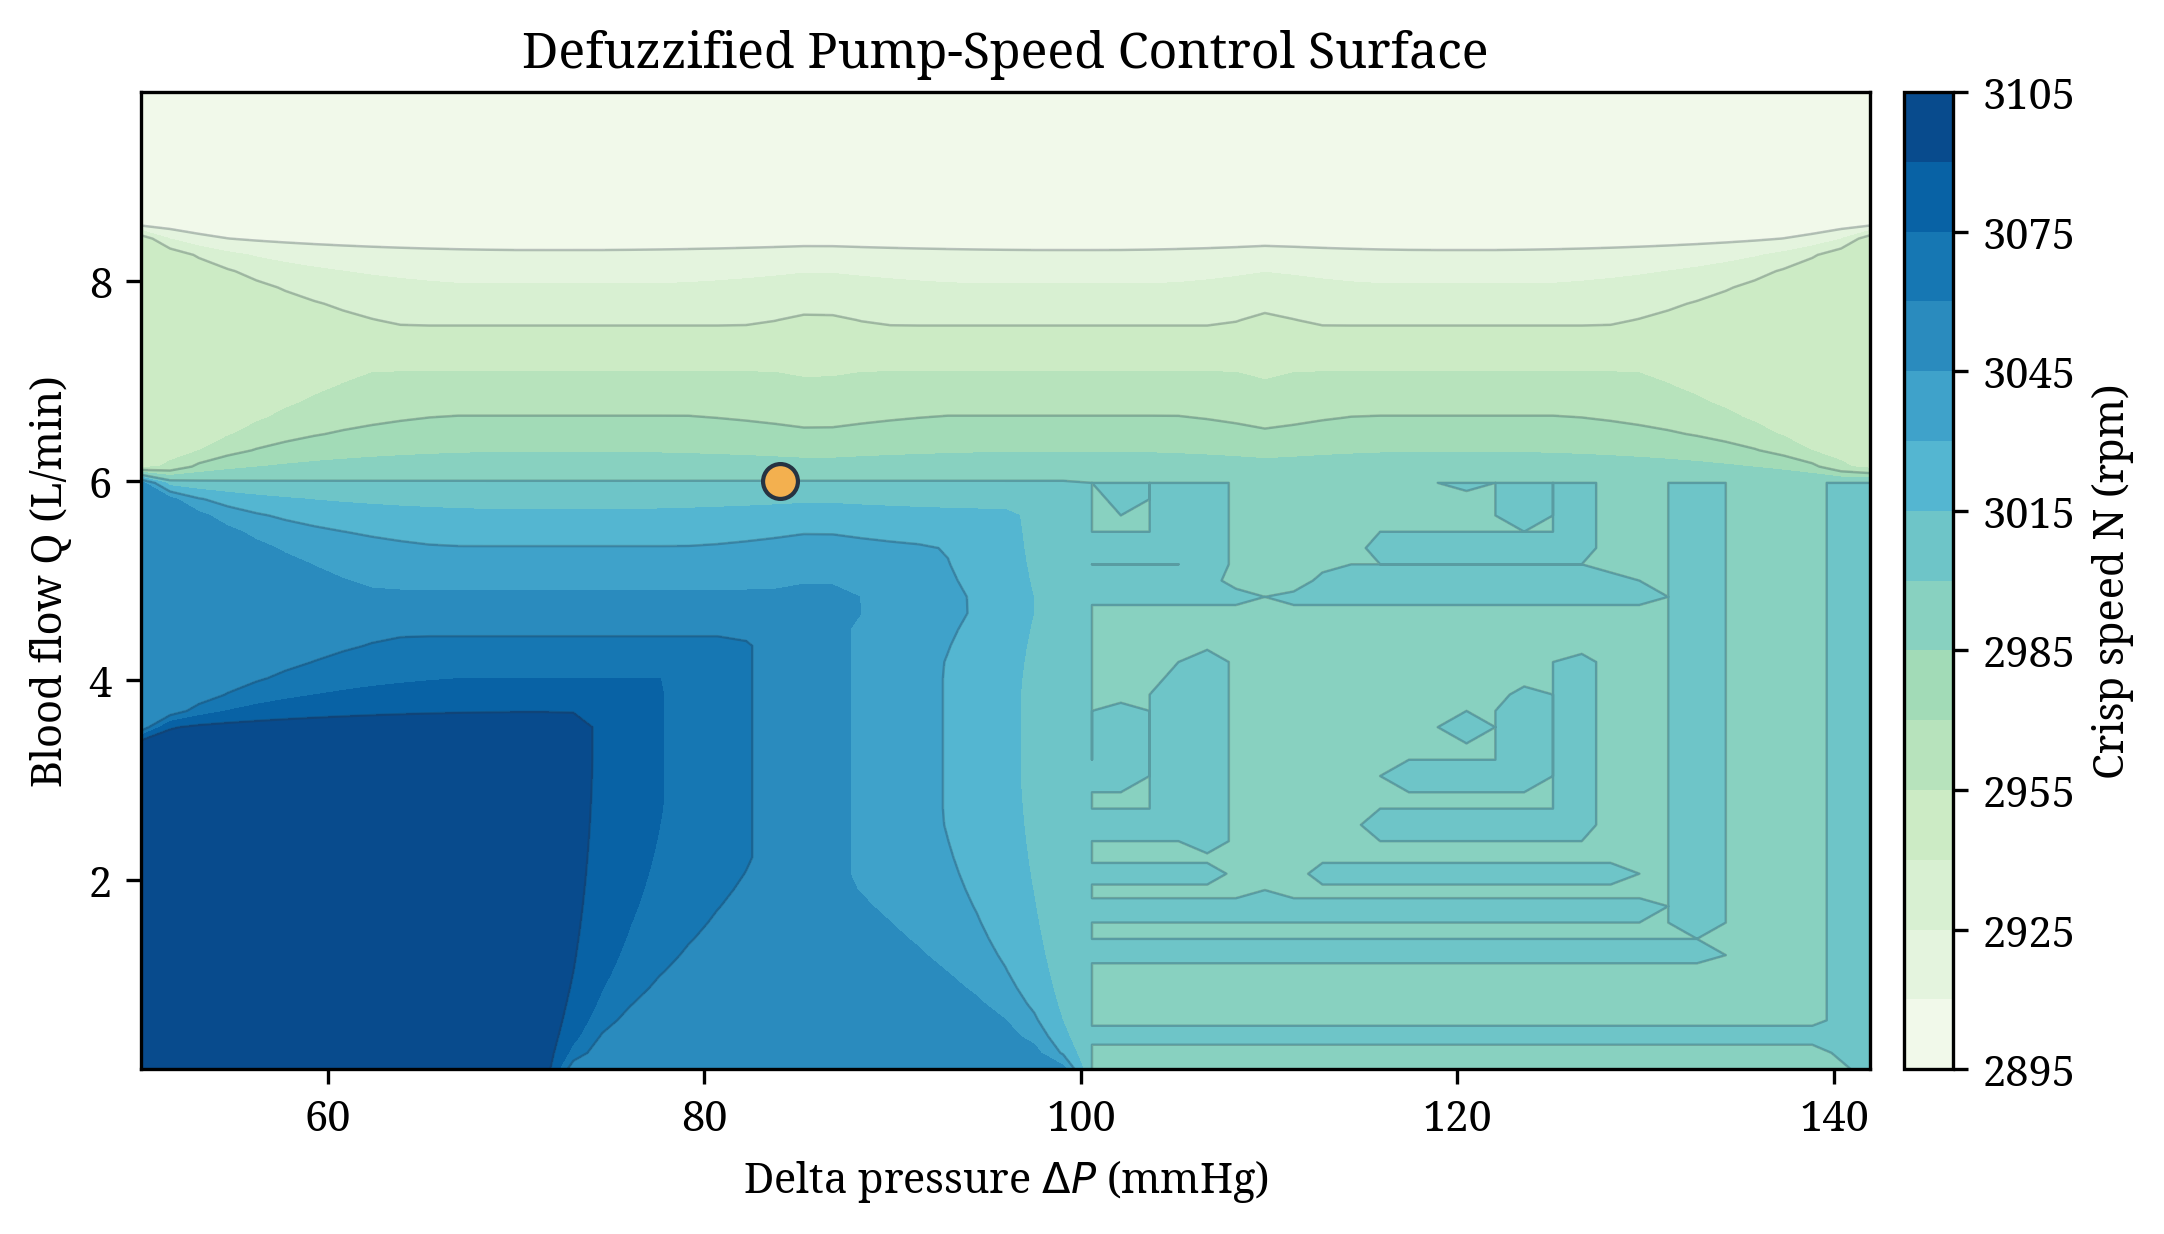
\includegraphics[width=0.46\linewidth]{control_surface.png}
  \captionof{figure}{Defuzzified control surface with the required operating point highlighted.}
\end{center}

Figure 4 is a broader check of the controller behavior over the input space. Each point on the surface is obtained by running the same fuzzy inference and centroid calculation for a different pair of \((\Delta P,Q)\). The highlighted point corresponds to the assignment case, showing where the computed \(3000\) rpm result sits relative to nearby operating conditions.

\section{Conclusion}

At \(\Delta P=84\) mmHg and \(Q=6\) L/min, the fuzzy controller activates the medium-speed consequent only. After aggregation and centroid defuzzification, the recommended rotary-pump speed is
\[
  \boxed{3000\ \text{rpm}}.
\]
This value is consistent with the controller goal of maintaining the reference flow near \(6\) L/min under moderate pressure loading. The Python file documents the computational workflow used for the fuzzy inference and defuzzification results in this report.

\end{document}
